%% For double-blind review submission, w/o CCS and ACM Reference (max submission space)
% \documentclass[sigplan,10pt,review,anonymous]{acmart}\settopmatter{printfolios=true,printccs=false,printacmref=false}
% \settopmatter{printacmref=false} % Removes citation information below abstract
% \renewcommand\footnotetextcopyrightpermission[1]{} % removes footnote with conference information in first column
% \pagestyle{plain} % removes running headers

%% For double-blind review submission, w/ CCS and ACM Reference
%\documentclass[sigplan,review,anonymous]{acmart}\settopmatter{printfolios=true}
%% For single-blind review submission, w/o CCS and ACM Reference (max submission space)
%\documentclass[sigplan,review]{acmart}\settopmatter{printfolios=true,printccs=false,printacmref=false}
%% For single-blind review submission, w/ CCS and ACM Reference
%\documentclass[sigplan,review]{acmart}\settopmatter{printfolios=true}
%% For final camera-ready submission, w/ required CCS and ACM Reference
\documentclass[sigplan,screen]{acmart}


%% Conference information
%% Supplied to authors by publisher for camera-ready submission;
%% use defaults for review submission.
\startPage{1}
\setcopyright{none}
\acmPrice{}
\acmDOI{10.1145/3385412.3386005}
\acmYear{2020}
\copyrightyear{2020}
\acmSubmissionID{pldi20main-p407-p}
\acmISBN{978-1-4503-7613-6/20/06}
\acmConference[PLDI '20]{Proceedings of the 41st ACM SIGPLAN International Conference on Programming Language Design and Implementation}{June 15--20, 2020}{London, UK}
\acmBooktitle{Proceedings of the 41st ACM SIGPLAN International Conference on Programming Language Design and Implementation (PLDI '20), June 15--20, 2020, London, UK}

%% Bibliography style
\bibliographystyle{ACM-Reference-Format}
%% Citation style
%\citestyle{acmauthoryear}  %% For author/year citations
%\citestyle{acmnumeric}     %% For numeric citations
%\setcitestyle{nosort}      %% With 'acmnumeric', to disable automatic
                            %% sorting of references within a single citation;
                            %% e.g., \citep{Smith99,Carpenter05,Baker12}
                            %% rendered as [14,5,2] rather than [2,5,14].
%\setcitesyle{nocompress}   %% With 'acmnumeric', to disable automatic
                            %% compression of sequential references within a
                            %% single citation;
                            %% e.g., \citep{Baker12,Baker14,Baker16}
                            %% rendered as [2,3,4] rather than [2-4].


%%%%%%%%%%%%%%%%%%%%%%%%%%%%%%%%%%%%%%%%%%%%%%%%%%%%%%%%%%%%%%%%%%%%%%
%% Note: Authors migrating a paper from traditional SIGPLAN
%% proceedings format to PACMPL format must update the
%% '\documentclass' and topmatter commands above; see
%% 'acmart-pacmpl-template.tex'.
%%%%%%%%%%%%%%%%%%%%%%%%%%%%%%%%%%%%%%%%%%%%%%%%%%%%%%%%%%%%%%%%%%%%%%

%% Other packages
\usepackage{algorithm}
\usepackage[noend]{algpseudocode}
\usepackage{algorithmicx}
\usepackage{tikz}
\usetikzlibrary{positioning,shadows,arrows,trees,shapes,fit}
\usepackage{pgfplots}
\pgfplotsset{compat=1.12}
\usepackage{pgfplotstable}
\usepackage{bm}
\usepackage{framed}
\usepackage{amsmath}
\usepackage{amssymb}
\usepackage{xspace}
\usepackage{listings}
\usepackage[skip=4pt]{caption}
\usepackage{microtype}

\lstset{
  language=Caml,
  basicstyle=\ttfamily,
  keywordstyle=\ttfamily,
}

\lstnewenvironment{code}{
\lstset{
  language=Caml,
  basicstyle=\ttfamily,
  keywordstyle=\ttfamily,
}}
{}

\lstnewenvironment{ecode}{
\lstset{
  language=Caml,
  basicstyle=\small\ttfamily,
  keywordstyle=\ttfamily\bfseries,
  numbers=left,
  xleftmargin=5.5mm,
  moredelim=[is][\bfseries]{==}{==},
  moredelim=[is][\underbar]{__}{__},
  moredelim=[is][\bfseries\underbar]{_=}{=_},
  escapeinside={(*@}{@*)}
}}
{}

\lstnewenvironment{compactcode}{
\lstset{
  language=Caml,
  basicstyle=\small\ttfamily,
  keywordstyle=\ttfamily\bfseries,
  xleftmargin=0mm,
  moredelim=[is][\bfseries]{==}{==},
  moredelim=[is][\underbar]{__}{__},
  moredelim=[is][\bfseries\underbar]{_=}{=_},
  escapeinside={(*@}{@*)}
}}
{}

\lstnewenvironment{haskellcode}{
\lstset{
  language=haskell,
  basicstyle=\small\ttfamily,
  keywordstyle=\ttfamily\bfseries,
  moredelim=[is][\bfseries]{==}{==},
  moredelim=[is][\underbar]{__}{__},
  moredelim=[is][\bfseries\underbar]{_=}{=_},
  escapeinside={(*@}{@*)}
}}
{}

\MakeRobust{\Call}

\newcommand{\algorithmautorefname}{Algorithm}

\lstMakeShortInline[mathescape=true]{|}

%% Our commands
\usepackage{commands}

%% Some recommended packages.
\usepackage{booktabs}   %% For formal tables:
                        %% http://ctan.org/pkg/booktabs
\usepackage{subcaption} %% For complex figures with subfigures/subcaptions
                        %% http://ctan.org/pkg/subcaption


\begin{document}

%% Title information
% \title[\toolname]{\toolname: Repairing Incorrect \\ Programming Assignment Solutions}
\title[\toolname]{Type Error Feedback via Analytic Program Repair}
% \titlenote{with title note}             %% \titlenote is optional;
%                                         %% can be repeated if necessary;
%                                         %% contents suppressed with 'anonymous'
% \subtitle{Subtitle}                     %% \subtitle is optional
% \subtitlenote{with subtitle note}       %% \subtitlenote is optional;
%                                         %% can be repeated if necessary;
%                                         %% contents suppressed with 'anonymous'
%% Author information
%% Contents and number of authors suppressed with 'anonymous'.
%% Each author should be introduced by \author, followed by
%% \authornote (optional), \orcid (optional), \affiliation, and
%% \email.
%% An author may have multiple affiliations and/or emails; repeat the
%% appropriate command.
%% Many elements are not rendered, but should be provided for metadata
%% extraction tools.

\author{Georgios Sakkas}
% \authornote{with author1 note}          %% \authornote is optional;
%                                         %% can be repeated if necessary
% \orcid{nnnn-nnnn-nnnn-nnnn}             %% \orcid is optional
\affiliation{
  % \position{Position1}
  \department{Computer Science \& Engineering}
  \institution{University of California, San Diego}
  % \streetaddress{Street1 Address1}
  \city{La Jolla}
  \state{CA}
  % \postcode{Post-Code1}
  \country{USA}
}
\email{gsakkas@eng.ucsd.edu}

\author{Madeline Endres}
\affiliation{
  \department{Computer Science \& Engineering}
  \institution{University of Michigan}
  \city{Ann Arbor}
  \state{MI}
  \country{USA}
}
\email{endremad@umich.edu}

\author{Benjamin Cosman}
\affiliation{
  \department{Computer Science \& Engineering}
  \institution{University of California, San Diego}
  \city{La Jolla}
  \state{CA}
  \country{USA}
}
\email{blcosman@eng.ucsd.edu}

\author{Westley Weimer}
\affiliation{
  \department{Computer Science \& Engineering}
  \institution{University of Michigan}
  \city{Ann Arbor}
  \state{MI}
  \country{USA}
}
\email{weimerw@umich.edu}

\author{Ranjit Jhala}
\affiliation{
  \department{Computer Science \& Engineering}
  \institution{University of California, San Diego}
  \city{La Jolla}
  \state{CA}
  \country{USA}
}
\email{jhala@cs.ucsd.edu}

\begin{abstract}
We introduce Analytic Program Repair, a data-driven
strategy for providing feedback for type-errors via
repairs for the erroneous program.
%
Our strategy is based on
insight that similar errors have similar repairs.
Thus, we show how to use a training dataset of
pairs of ill-typed programs  and their fixed versions to:
%
(1)~\emph{learn} a collection of candidate repair templates
    by abstracting and partitioning the edits made in the
    training set into a representative set of templates;
%
(2)~\emph{predict} the appropriate template from a given error,
    by training multi-class classifiers on the repair templates
    used in the training set;
%
(3)~\emph{synthesize} a concrete repair from the template
   by enumerating and ranking correct (\eg well-typed)
   terms matching the predicted template.
%
We have implemented our approach in \toolname: a type error reporting
tool for \ocaml programs. We present an evaluation of the
\emph{accuracy} and \emph{efficiency} of \toolname on a corpus
of 4,500 ill-typed \ocaml programs drawn from two instances of an
introductory programming course, and a user-study of the \emph{quality}
of the generated error messages that shows the locations and
final repair quality to be better than the state-of-the-art tool
in a statistically-significant manner.
\end{abstract}


%% 2012 ACM Computing Classification System (CSS) concepts
%% Generate at 'http://dl.acm.org/ccs/ccs.cfm'.
\begin{CCSXML}
<ccs2012>
<concept>
<concept_id>10011007.10011006.10011008</concept_id>
<concept_desc>Software and its engineering~General programming languages</concept_desc>
<concept_significance>500</concept_significance>
</concept>
<concept>
<concept_id>10003456.10003457.10003521.10003525</concept_id>
<concept_desc>Social and professional topics~History of programming languages</concept_desc>
<concept_significance>300</concept_significance>
</concept>
</ccs2012>
\end{CCSXML}

\ccsdesc[500]{Software and its engineering~General programming languages}
\ccsdesc[300]{Social and professional topics~History of programming languages}
%% End of generated code


%% Keywords
%% comma separated list
% \keywords{keyword1, keyword2, keyword3}  %% \keywords are mandatory in final camera-ready submission


%% \maketitle
%% Note: \maketitle command must come after title commands, author
%% commands, abstract environment, Computing Classification System
%% environment and commands, and keywords command.
\maketitle

\section{Introduction}
\label{sec:intro}

%%% Motivation and the problem
The increasing number of computer science related
jobs~\citep[][]{compsci-demand} in the recent years has resulted in an
unprecedented demand for computer science education. Colleges and universities
have more students than ever~\citep[][]{compsci-classes} enrolled to their
computer science classes and their numbers will only increase in the foreseeable
future. Other students wanting to join this growth of technology and computing,
have turned to Massive Open Online Courses (MOOCs)~\citep[][]{moocs} to get the
appropriate knowledge in order to pursue their dream in the technology job
market. While computer science education has become much more accessible with
these larger classrooms over the years, one may ask if its \emph{quality} has
remained the same as of the more traditional smaller classrooms, and
specifically the feedback that students get for homework and exams.

%%% Good properties of a solution
Recent research has focused on providing \emph{fully automated feedback} to
students for the programming assignments that these classes usually include. In
this paper we propose such a solution, that can be used to give personalized
feedback to students for introductory programming exercises without requiring
any instructor effort. Previous work has exploited the advances in \emph{program
repair} research to generate such feedback.
% TODO: Cite clara, autoproof, sarfgen, ... here

By repairing an incorrect student attempt on a programming assignment and
producing a \emph{minimal} repair \wrt some edit-distance metric, so it can be
as close as possible to the original one, we can generate \emph{high-quality}
feedback for that attempt. Furthermore, the repair algorithm we propose must be
able to \emph{generalize} over different programming assignments and to not be
specific to existing ones only. In this paper we focus on generating such
repairs that will enable better feedback generation and leave the latter part as
future work.

%%% Current state of the art
% Failing test cases
Presenting students with \emph{failing test cases} still remains one of the most
common approaches for providing feedback on erroneous programming assignments
attempts. These test cases can be carefully selected by the instructor to guide
their students in debugging their code. However, for students that are not yet
so experienced in programming, such feedback may not be sufficient. More
targeted feedback is needed in this case, that will highlight possible program
locations that are responsible for the program errors, and may give possible
suggestions that will lead the student to a correct solution.

% Fault localization FIXME: make this better
Recent research~\citep[][]{Seidel:2017, Zhang2014-lv} has proposed the use of
\emph{fault localization} for more guided feedback. Fault localization is the
task of identifying possible program elements (\eg lines, expressions \etc) that
are the cause of the program error at hand. While these techniques can pinpoint
with high accuracy the precise location in the student's code that cause the
error and needs to be fixed, inexperienced programmers can still be confused by
such feedback. However, fault localization combined with \emph{program repair}
can provide the appropriate feedback for those novice programmers.

% Program repair
Recent automated systems for providing feedback via \emph{program repair}, like
AutoGrader [TODO: cite] demand a lot of manual effort from the instructor and
their understanding of the system details. AutoGrader requires a reference
solution per programming assignment and a custom error model that will help
repair incorrect student attempts, thus the instructor has to spent extra time
for each assignment, while the algorithm finding the repairs is still very
expensive due to constraint-solving. Systems like CLARA [TODO: cite] require
much less manual effort from the instructor by using clustering and machine
learning techniques on previous student attempts on the programming assignments.
While the repairs are generated relatively quickly, their program matching
between previous correct attempts and the new incorrect ones, can often lead to
imprecise and not minimal repairs. Moreover, their use of Integer Linear
Programming (ILP) for variable alignment between possible local repairs can hurt
its scalability. [TODO: Section N] provides a detailed survey of related work.
% TODO: Add Seminal(it's the one on our human study) here?
% TODO: Maybe add another tool?

% FIXME: help here!!
%%% Our technique
\mypara{Data-Driven Program Repair}
In this paper, we introduce \toolname, a \emph{data-driven} approach to
repairing novice attempts on programming assignments based on supervised
learning. \toolname uses a large dataset with pairs of ill-typed programs and
their subsequent fixes, to \emph{automatically learn models} that localize
errors, suggest template fixes, and uses \emph{program synthesis} to turn those
templates into \emph{program repairs}. Given a new ill-typed program, \toolname
generates a list of potential solutions ranked by likelihood and a
\emph{edit-distance} metric. We evaluate \toolname by comparing its accuracy on
a set of over 4,500 ill-typed \ocaml programs drawn from two instances of an
introductory programming course.


% 1. ``We identify an important problem in the world.'' Be more specific than
% just ``bugs''. Are we focusing on novices and students or are we focusing
% on general software defects? Are we focusing on strongly-typed functional
% languages or are we proposing something generic? What ``news article'' or
% ``survey paper'' citations can you list here to convince me that this is a
% big deal?

% 2. ``Here are the properties that a good solution must have.'' Pick three.
% Here are some examples: must be applicable to students; must produce
% answers quickly; must produce answers that are very close to what humans
% would do; must apply to programs from a wide range of application domains.

% 3. ``Here is the current state of the art. Note that each of these fails to
% obtain at least one of the properties above.'' Candidates: manual debugging
% (bad because of X and Y); using something like genprog (bad because of X
% and Z); using pure fault localization (bad because of A and B); using delta
% debugging or git/svn blame (bad because of P and Q); using something like
% Nate or Sherrloc (bad because of Q and R).

% 4. ``Here are our two or three insights. These insights are the
% underpinning of our solution.'' What are the most important ones?
% Candidates: blame-labeled training sets are available; student repairs fall
% into a reasonable number of categories (admitting a classification
% technique); program repair can be viewed as a synthesis problem;
% generalized ASTs can handle typed and untyped program manipulations.

% 5. ``We combine those insights into TECHNIQUE. It works by steps A, B and
% C, which allow it to obtain the properties P1, P2, and P3 of a good
% solution.'' Briefly condense the steps from Section 2 here.

% 6. ``We evaluate our technique. For Property P1, we use metric M1 and must
% be at least as good as S1 to be successful. For Property P2, we use metric
% M2 and must be at least as good as S2 to be successful. We obtain property
% P3 by construction.'' Fill in the blanks. In addition, for every benchmark
% set or human study used, indicate why you are sampling correctly --- why
% those results are likely to generalize.

% The contributions of this paper are as follows:
% \begin{itemize}
%   \item The algorithm. FIXME.
%   \item The dataset. FIXME --- is this a contribution?
%   \item The empirical evaluation. FIXME.
%   \item The human study. FIXME.
% \end{itemize}


\section{Overview}
\label{sec:overview}


We begin with an overview of our approach to suggesting fixes for various faulty
programs by collectively learning from the processes novice programmers take to
fix errors in their programs.

\begin{figure}[ht]
    \begin{ecode}
      let rec mulByDigit i l =
        match l with
        | []     -> []
        | hd::tl -> (hd * i) @ (mulByDigit i tl)
    \end{ecode}

    \begin{ecode}
      let rec mulByDigit i l =
        match l with
        | []     -> []
        | hd::tl -> [hd * i] @ (mulByDigit i tl)
    \end{ecode}
    \caption{(top) An ill-typed \ocaml program that should multiply each element
    of a list with an integer. (bottom) The fixed version by the student.}
    \label{fig:mulByDigit}
\end{figure}


\mypara{The Problem.} Consider the \texttt{mulByDigit} program in
\autoref{fig:mulByDigit} written by a student in an undergraduate Programming
Languages course. The program is meant to multiply all the numbers in a list
with an integer digit, but the student accidentally misuses the list append
operator (\texttt{@}), applying it to a number and a list rather than two lists.
Novice programmers may not find the compiler's resulting type checking error
message informative.  In this particular instance, the student chose the
approach shown in \autoref{fig:mulByDigit}, but multiple solutions are possible,
including using the \texttt{::} operator to prepend a single element onto a
list. We desire an automated technique to guide novice programmers by suggesting
candidate solutions.

\mypara{Solution. Suggesting Repairs via Supervised Classification and Program
Synthesis.} Our approach is to view the process of \emph{fixing} an erroneous
program as a \emph{supervised multi-class classification problem}, whose results
are then fed to a \emph{program synthesizer}. A classification problem entails
learning a function that maps inputs to a discrete set of output labels (in
contrast to techniques such as regression, where the output is typically a real
number). A supervised learning problem is one in with an available training set
where the inputs and labels are known, and the task is to learn a function that
accurately maps the inputs to output labels and generalizes to future inputs. To
realize the above approach for suggesting good possible repairs as a practical
tool, we structure our solution into five sub-problems:

\begin{enumerate}
  \item How can we acquire a training set of labeled ill-typed programs with
  their respective user-provided fixes?
  \item How can we represent possible solutions to a defect?
  \item What are the appropriate models to represent this problem?
  \item How can we use predictive models to repair faulty programs?
  \item How can we use predictive models and synthesized repairs to give
  localized feedback to the programmer?
\end{enumerate}

In the remainder of this section, we consider each sub-problem in turn.

%%% FIXME: Taken mostly from Nate, needs many changes...
\subsection{Step 1: Acquiring a Blame-Labeled Training Set}
\label{subsec:step1}

The first step is to gather a training set of ill-typed programs, where each
erroneous sub-term is explicitly labeled. Prior work has often enlisted expert
users to curate a set of ill-typed programs and then \emph{manually} determine
the correct fix~\citep[\eg][]{Lerner2007-dt, Loncaric2016-uk}. This method is
suitable for evaluating the quality of a localization (or repair) algorithm on a
small number (e.g. 10s--100s) of programs. However, in general it requires a
great deal of effort for the expert to divine the original programmer's
intentions. Consequently, is difficult to scale the expert-labeling to yield a
dataset large enough (e.g. 1000s of programs) to facilitate machine learning.
More importantly, this approach fails to capture the frequency with which errors
occur in practice.

\mypara{Interaction Traces.} We solve both the scale and frequency problems by
instead extracting blame-labeled data sets from \emph{interaction traces}.
Software development is an iterative process. Programmers, perhaps after a
lengthy (and sometimes frustrating) back-and-forth with the type checker,
eventually end up fixing their own programs. Previous work has used an
instrumented \ocaml compiler to record this conversation, i.e. record the
sequence of programs submitted by each programmer and whether or not it was
deemed type-correct. For each ill-typed program in a particular programmer's
trace, they find the first subsequent program in the trace that type checks and
declare it to be the fixed version. In our case, we used an existing extracted
dataset~\citep[][]{yunounderstand, Seidel:2017} of ill-typed programs and their
fixes. From these pairs, we can extract a \emph{diff} of the abstract syntax
trees (ASTs), and then assign the blame labels to the \emph{smallest} sub-tree
in the diff.

\mypara{Example.} Suppose our student fixed the \texttt{mulByDigit} program as
shown above by adding a \texttt{[]} around the result of the multiplication, the
diff would include the list expression. Thus we would determine that the list
expression is the repair we have to blame.

\mypara{Bags-of-Abstracted-Terms.} Our representation of programs is
parameterized by a set of feature abstraction functions, (abbreviated to feature
abstractions) $f_1, \ldots, f_n$ , that map terms to a numeric value (or just
$\{0, 1\}$ to encode a boolean property). Given a set of feature abstractions,
we can represent a single program's AST as a \emph{bag-of-abstracted-terms}
(BOAT) by:
%
(1) decomposing the AST (term) $t$ into a bag of its constituent sub-trees
(terms) $\{t_1, \ldots, t_m\}$; and then
%
(2) representing each sub-term $t_i$ with the $n$-dimensional vector $[f_1(t_i),
\ldots, f_n(t_i)]$. Working with ASTs is a natural choice as type-checkers
operate on the same representation.

\mypara{Modeling Contexts.} Each expression occurs in some surrounding
\emph{context}, and we would like the classifier to be able make decisions based
on the context as well. The context is particularly important for our task as
each expression imposes typing constraints on its neighbors. For example, a |@|
operator tells the type checker that both children must have type |'a list| and
that the parent must accept an |'a list|. The BOAT representation makes it easy
to incorporate contexts: we simply \emph{concatenate} each term’s feature vector
with the \emph{contextual features} of its parent and children.

\mypara{Type features.} Another way to summarize the context in which an
expression occurs is with types. Of course, the programs we are given are
untypeable, but we can still extract a partial typing derivation from the type
checker and use it to provide more information to the model. However, to help
later our classifier give better predictions of the possible fixes, we want
those types to be as close as possible to the types that correct program would
have or at least be a super-type of them. To achieve that, we replace each time
one location of the program with a typed hole and extend the type checker to
infer the type of that hole from the context of the program. This procedure
would give more accurate super-types than getting partial typing derivation from
the untypeable original program.



\subsection{Step 2: Representing fixes as labels}
\label{subsec:step2}

Next, we represent different fixes via a limited number of templates. We focus
on AST-level templates that are easy for novices to understand.

\mypara{Clustering the Fixes.} Our dataset contains erroneous programs and the
corresponding user-written fixes. Those fixes can be arbitrary code
modifications with different lengths, variable names, functions, and so on. We
propose to automatically cluster such fixes into abstract fix schema. This
clustering serves two purposes. First, it enables the subsequent use of discrete
classification algorithms to choose. Second, it allows for the principled
removal of outliers. Outliers are a relevant problem because student datasets
often contain non-standard or idiosyncratic solutions. We propose to use a
simple clustering algorithm applied atop a similarity metric for fixes.
%
% FIXME: The original text had \emph{equivalent} here. Do you actually mean
% that? If so, be more precise. The text also talked about outlier removal,
% so I made that more formal --- but is it something we're actually doing?

\mypara{Generic Abstract Syntax Trees.}
Fixes in our dataset are represented as the ASTs of the expressions that changed
in the ill-typed programs and transformed the program to the correct solution.
To enable \emph{similar fixes} in different ill-typed programs to be clustered
together and thus get a smaller number of clusters of better quality, we propose
a further simplification of the changed ASTs: the Generic Abstract Trees
(GASTs). GASTs are taken from their respective ASTs, with all the specific
variable, function, operator and etc. names removed from them. These trees keep
information only about the \emph{structure} of the fix rather than the specific
changes in variables and functions. We also prune these GASTs at a certain depth
$d$ to keep only the top-level changes of the fix. Pruned sub-trees are replaced
with \emph{holes}, which represent that \emph{any expression} is possible to
fill them.

% TODO: Make figure of GAST for running example.
% The ASTs of the fixes is a good start, but those still contain too much
% information. See our running example. |[hd * i]| is a list that includes a
% multiplication of the variables |hd| and |i|. While we care about the list and
% the binary operator, all the rest information is not that important. T

\mypara{Fix Templates.} Previous work~\citep[][]{martinez2013automatically,
martinez2015mining} has used \emph{fix templates} to generate \emph{patches}
that can be used to repair an erroneous program. Those templates are usually
picked manually by inspecting a large corpus of buggy programs and their fixes.
However, we show that such fix templates can be \emph{learned} from those
datasets using the clusters of fixes' GASTs. A GAST representative of a cluster
can be used as a fix template in order to produce a fix or provide feedback for
the type-error that a faulty program raises.

% TODO: Show template for running example.
% For our example, the GAST would be a list with a binary operator as a child,
% whose children in return would be holes, if we were to prune GASTs at a depth $d
% = 2$. The binary operator would also be unknown at this point, thus creating a
% template of the form |[_ # _]|. We see in \autoref{fig:suggestion} how that
% template would work to provide feedback to programmers, but we discuss later how
% we can complete the template with program synthesis.

\begin{figure}[ht]
  \begin{ecode}
    let rec mulByDigit i l =
      match l with
      | []     -> []
      | hd::tl -> [_ # _] @ (mulByDigit i tl)
  \end{ecode}
  \caption{A possible template for the \texttt{mulByDigit} program.}
  \label{fig:suggestion}
\end{figure}



\subsection{Step 3: Training Predictive Models}
\label{subsec:step3}

Now we have a minimal set of fix templates that we want to predict from. We
enumerate our templates, starting from 1, and update the dataset to have as
labels the number of the template that \emph{fixes} that location of the
program. We can now train a classifier that predicts fix templates given a
ill-typed program. Because we still have multiple templates (\emph{classes}) to
choose from, we have a multi-class problem in our hands, as opposed to the more
common binary classification. We will treat error localization as binary
classification problem.

\mypara{Error Localization.} Previous work has shown to give excellent accuracy
on localizing type-errors using program analytics techniques. In order to reduce
the complexity of predicting the correct template and the location that it
should be applied from our multi-class classifier, we separate those two
problems. We use a second DNN classifier to associate locations with their
probability to be fixed. Then, starting from the locations with the highest
probabilities to be fixed, we try to repair them using the template predictions
for those particular locations.

\mypara{Multi-class Classification.} We choose models that can handle multiple
classes as labels. Such models are Deep Neural Networks (DNNs). But those models
produce not only a predicted template-class, but they also associate a metric
that can be interpreted as the classifier’s confidence in its prediction. We use
deep and dense architectures to give a better confidence to each template, with
more accuracy.



\subsection{Step 4: Program Repair}
\label{subsec:step4}

After making template predictions and error localization for ill-typed programs,
we exploit existing program synthesis techniques to fill holes and generic
expressions that our templates have and return programs that type-check. This
way, we can also eliminate templates that wouldn’t actually work for a
particular location.

\mypara{Program Synthesis.} Given a set of locations and candidate templates for
those locations, we are trying to solve a problem of synthesis, meaning that we
try to generate code that would match the template’s GAST and make the program
type-check. For each location, we enumerate all possible expressions, until we
find a small set that makes the program to type-check. We try to use existing
code in our synthesis algorithm, by considering subexpressions of the
expressions we try to replace.

\mypara{Synthesis for Multiple Locations.} Using our error localization
predictions, we get a confidence for each location in the type-error slice.
Previous work has shown that just the top 3 locations from this set can solve up
to 90\% of type-errors. But there are cases where more than one location needs
to be fixed. Therefore, we rank the confidence of the powerset of all locations.
The confidence for a subset of locations can be acquired by the product of each
location’s confidence in the subset. This holds because we consider each
location’s probability to be the correct location to be fixed independent from
other locations.



\subsection{Step 5: Generating Feedback}
\label{subsec:step5}

Finally, having generated automatic repairs for a given ill-typed program using
our predictive models and program synthesis, we want to use that to help users
completely fix their programs and understand what the problem was in the
original program. To do so, we want to provide \emph{minimal} repairs to
students, meaning repairs that are as close to their original program but also
catch the programmers intent for that piece of code. Since we have multiple fix
templates to choose from and many candidate locations to fix in a program, maybe
the user would find it most useful to get more than one suggestion, and those
suggestions to be ranked according to some metric.

\mypara{Ranking Fixes.} We rank each solution by two metrics, the
\emph{tree-edit distance} and the \emph{string-edit} distance. Previous work has
used those metrics to consider minimal changes, i.e. changes that are as close
as possible to the original programs, so novice programmers can better
understand feedback. However, different metrics may give betters fixes as we
discuss later. Programmers usually have in mind what the \emph{type signature}
the functions that they write are supposed to have. So, it is reasonable to
provide the option to the user to give the intended type for the program's
functions we are trying to repair. In our case, we acquire the intended types
from the fixed versions of the dataset.

\mypara{Example.} In \autoref{fig:repair} we can see a minimal repair that our
method could return, using the template and error location discussed in
\autoref{subsec:step2} to synthesize this solution. However, this solution is
not the top one that are implementation would give (that would be identical to
the solution the programmer gave), we use this repair to demonstrate different
aspects of the synthesizer. We can see that this solution is very close to the
one that the programmer finally came up with, but still has some holes. This
time, however, there are some indications as to what these holes should be. Here
our synthesizer suggested two different variables should be used to fill those
template holes.

\begin{figure}[ht]
  \begin{ecode}
    let rec mulByDigit i l =
      match l with
      | []     -> []
      | hd::tl -> [_var1_ * _var2_] @ (mulByDigit i tl)
  \end{ecode}
  \caption{A candidate repair for the \texttt{mulByDigit} program.}
  \label{fig:repair}
\end{figure}

\section{Learning Fix Templates}
\label{sec:templ-partition}

We start by introducing our approach for extracting useful \emph{fix templates}
from a training dataset comprising of erroneous-and-fixed programs.
%
We express those templates in terms of a language that allow us to succinctly
represent fixes in a way that captures the essential structure of various fix
patterns that novices use in practice.
%
However, extracting a single fix template for \emph{each} fix in the program
pair dataset yields too many templates to perform accurate predictions.
%
Hence, we define a \emph{similarity} relation between templates, which we use to
\emph{partition} the extracted templates into a smaller set, that will make it
easier to train precise models to predict fixes.

\begin{figure}
\small
\centering
  \begin{minipage}[c]{\linewidth}
  \[
  \boxed{
  \begin{array}{rcl}
  e & ::=    & x \spmid \efun{x}{e} \spmid \eapp{e}{\bar{e}} \spmid \elet{x}{e}{e} \\
    & \spmid & n \spmid b \spmid \eplus{e}{e} \spmid \eif{e}{e}{e} \\
    & \spmid & \epair{e}{e} \spmid \epcase{e}{x}{x}{e} \\
    & \spmid & \enil \spmid \econs{e}{e} \spmid \ecase{e}{e}{x}{x}{e} \\[0.05in]

  n & ::= &  0, 1, -1, \ldots \\[0.05in]

  b & ::= &  \etrue \spmid \efalse \\[0.05in]

  t & ::= & \alpha \spmid \tbool \spmid \tint \spmid \tfun{t}{t} \spmid \tprod{t}{t} \spmid \tlist{t} \\[0.05in]
  \end{array}
  }
  \]
  \captionof{figure}{Syntax of \lang}
  \label{fig:ml-syntax}
  \end{minipage}
  \begin{minipage}[c]{\linewidth}
    \[
    \boxed{
    \begin{array}{rcl}
    e & ::=    & \_  \spmid \hat{x} \spmid \efun{\hat{x}}{e} \spmid \eapp{\hat{x}}{\bar{e}} \spmid \elet{\hat{x}}{e}{e} \\
      & \spmid & \hat{n} \spmid \ebop{e}{e} \spmid \eif{e}{e}{e} \\
      & \spmid & \epair{e}{e} \spmid \epcase{e}{\hat{x}}{\hat{x}}{e} \\
      & \spmid & \enil \spmid \econs{e}{e} \spmid \ecase{e}{e}{\hat{x}}{\hat{x}}{e} \\[0.05in]
    \end{array}
    }
    \]
    \captionof{figure}{Syntax of \repairLang}
    \label{fig:rtl-syntax}
  \end{minipage}
\end{figure}


\subsection{Representing User Fixes}
\label{sec:templ-partition:lang}

\paragraph{Repair Template Language.}
\autoref{fig:rtl-syntax} describes our Repair Template Language, \repairLang,
which is a lambda calculus with integers, booleans, pairs, and lists, that
extends our core ML language \lang (\autoref{fig:ml-syntax}) with several
syntactic abstraction forms:

\begin{enumerate}
    \item \emph{Abstract variable} names $\hat{x}$  are used to denote variable
    occurrences for functions, variables and binders, \ie $\hat{x}$ denotes
    an unknown variable name in \repairLang;

    \item \emph{Abstract literal} values $\hat{n}$ can represent \emph{any}
    integer or floating point number, boolean value or character and string;

    \item \emph{Abstract operators} $\oplus$ similarly denote unknown unary or
    binary operators;

    \item \emph{Wildcard} expressions $\_$ are used to represent \emph{any}
    expression in \repairLang, \ie a program \emph{hole}.
\end{enumerate}

Recall from \autoref{sec:overview:templates} that we define fixes as
replacements of expressions with new candidate expressions at specific program
locations. Therefore, we express candidate expressions over \repairLang as means
to represent our fix templates $\T$.

\paragraph{Generalizing ASTs.}
A \emph{Generic Abstract Syntax Tree} (GAST) is a term from \repairLang that
represents many possible expressions from \lang. GASTs are abstract from
standard ASTs over the core language \lang using the $\abstrsym$ function that
takes as input an expression $e^{ML}$ over \lang and a depth $d$ and returns an
expression $e^{RTL}$ over \repairLang, \ie a GAST with all variables, literals
and operators of $e^{ML}$ abstracted and all subexpressions starting at depth
greater than $d$ pruned and replaced with holes $\_$.

\begin{figure}
    \centering
    \begin{minipage}[c]{0.49\linewidth}
        \centering
        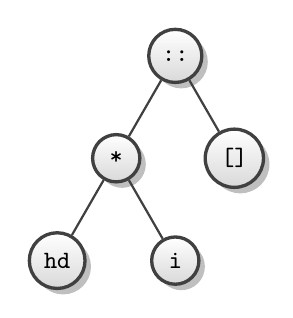
\begin{tikzpicture}
        [font=\small, edge from parent,
        every node/.style={top color=white, bottom color=black!15,
        circle, minimum size=6mm, draw=black!75,
        very thick, drop shadow, align=center},
        edge from parent/.style={draw=black!75,thick},
        level distance=1.3cm]
        \node (cons) {\texttt{::}}
            child { node (mult) {\texttt{*}}
                child { node {\texttt{hd}}}
                child { node {\texttt{i}}}
                }
            child {node (elist) {\texttt{[]}}};
        \end{tikzpicture}
        \subcaption{Fix AST}
        \label{fig:fix_ast}
    \end{minipage}
    \begin{minipage}[c]{0.49\linewidth}
        \centering
        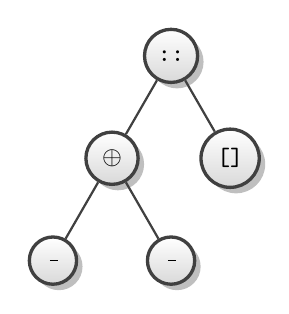
\begin{tikzpicture}
            [font=\small, edge from parent,
            every node/.style={top color=white, bottom color=black!15,
            circle, minimum size=6mm, draw=black!75,
            very thick, drop shadow, align=center},
            edge from parent/.style={draw=black!75,thick},
            level distance=1.3cm]
            \node (cons) {\texttt{::}}
                child { node (mult) {\texttt{$\oplus$}}
                    child { node {\texttt{$\_$}}}
                    child { node {\texttt{$\_$}}}
                    }
                child {node (elist) {\texttt{[]}}};
            \end{tikzpicture}
        \subcaption{Template GAST}
        \label{fig:templ_gast}
    \end{minipage}
    \caption{(left) The fix from example \autoref{fig:mulByDigit} and (right) a possible template for that fix. \GS{does this help? maybe move this to overview?}}
\end{figure}


\paragraph{Example.}
Recall our example program \mbd in \autoref{fig:mulByDigit}.
%
The expression |[hd * i]| replaces |(hd * i)| in line 4, and hence, is the
user's \emph{fix}, whose AST is given in \autoref{fig:fix_ast}.
%
The output of $\abstrsym$, given this AST and a depth $d = 2$ as input, would be
the GAST in \autoref{fig:templ_gast}, where the operator |*| has been replaced
with an abstract operator $\oplus$, and the sub-terms |hd| and |i| at depth 2
have been abstracted to wildcard expressions $\_$.
%
Hence, the \repairLang term |[_ $\oplus$ _]| represents a potential fix template
for \mbd.

\subsection{Extracting Fix Templates from a Dataset}
\label{sec:templ-partition:templates}

Our approach fully automates the extraction of fixes by harvesting a set of fix
templates from a training set of program pairs.
%
Given a program pair $(\pbad, \pfix)$ from the dataset, we extract a unique fix
for each location in $\pbad$ that changed in $\pfix$.
%
We do so with an expression-level $\diffsym$~\citep{Lempsink2009-xf} function.
%
Recall again that we consider fixes to be replacements of expressions, and
therefore we use the extracted changes as our fix templates.

\paragraph{Contextual Repairs.}
%
Following \cite{Felleisen92} let $\econtext{}$ be the \emph{context} that an
expression $e$ appears in a program $p$, \ie the program $p$ with expression $e$
replaced with a hole $\_$.
%
We write that $p = \context{}{e}$, meaning that if we fill the hole with the
original expression $e$ we obtain the original program $p$.
%
In this fashion, $\diffsym$ finds a \emph{minimal} (in number of nodes)
expression replacement $\efix$ for an expression $\ebad$ in $\pbad$, such that
$\pbad = \context{\pbad}{\ebad}$ and $\context{\pbad}{\efix} = \pfix$.
%
There may be several such expressions in a program, and $\diffsym$ returns all
such changes.

\paragraph{Example.}
If a new expression has been inserted \emph{around} an existing expression, \eg
if $\eapp{f}{x}$ is rewritten to $\eapp{g}{x}$, we will have that the context is
$\econtext{} = \eapp{\_}{x}$, where $\_$ represents the hole, and then the fix
will be $g$, since $\context{}{g} = \eapp{g}{x}$.

If instead, an expression has been replaced wholesale with another expression,
\eg if $\eapp{f}{x}$ is rewritten to $\eplus{(\eapp{f}{x})}{1}$, the
\emph{context} will be the more general $\econtext{} = \_$, since we consider
the application expression $\eapp{f}{x}$ (but not $f$ or $x$) to be replaced
with the $+$ operator, and therefore the fix will be the whole expression, thus
$\context{}{\eplus{(\eapp{f}{x})}{1}} = \eplus{(\eapp{f}{x})}{1}$.
% TODO: maybe talk about the drawback of the last choice

\subsection{Partitioning the Templates}

Programs over \lang force similar fixes, such as changes to variable names, to
have identical GASTs. Our next step is to define a notion of program fix
\emph{similarity}. Our definition supports the formation of a small but widely
applicable set of fix templates. This small set is used to train a repair
predictor.

\label{subsec:partitioning}
\begin{figure*}
\begin{minipage}{\textwidth}
\begin{haskellcode}
==data Expr== = Var | Bop Expr Expr | App [Expr] | Hole | ..

==sim :: Expr -> Expr -> Bool==
sim e           Hole        = True
sim Var         Var         = True
sim (Bop x1 y1) (Bop x2 y2) = sim [x1, x2] [y1, y2] ==||== sim [y1, y2] [x1, x2]
sim (App xs)    (App ys)    = any (\ys' -> any (\xs' -> sim xs' ys') xss) yss
    where
        xss = permutations xs
        yss = permutations ys
sim _           _           = False

==sim :: [Expr] -> [Expr] -> Bool==
sim (x:xs) (y:ys) = sim x y && sim xs ys
\end{haskellcode}
\end{minipage}
\caption{$\simil{e_1}{e_2}$ denotes when the GAST $e_1$ is similar to $e_2$.}
\label{fig:similar}
\end{figure*}

\paragraph{GAST Similarity.}
%
\autoref{fig:similar} formalizes a relation that states when
an expression $e_1$ is \emph{similar to} $e_2$  (written \simil{e_1}{e_2}).
%
Intuitively, $e_1$ is similar to $e_2$ when at least one of the following rules
hold
\begin{enumerate}
    \item every expression is similar to a wildcard $\_$;

    \item the top-level non-terminal is the same and there is a total bijective
        relation between their sub-expressions \st they are all pair-wise
        similar, \eg two binary operator expressions are the same if their
        operands are similar;
        % \eg $e_{11} \oplus e_{12}$ and $e_{21} \oplus e_{22}$ are
        % similar \textit{iff} $(e_{11}, e_{21})$ and $(e_{12}, e_{22})$ or
        % $(e_{11}, e_{22})$ and $(e_{12}, e_{21})$ are pair-wise similar.

    \item a terminal expression is similar to another, only when they are the
    same, \eg two variables are similar.
\end{enumerate}
%


% TODO: partition is novel? compare to previous work
\paragraph{Partitioning.}
The GAST similarity we defined is both symmetric and transitive and thus is an
\emph{equivalence} relation. We can now define \emph{partitioning} as the
computation of all possible \emph{equivalence classes} of our extracted fix
templates \wrt our GAST similarity relation. Each class can consist of several
member-expressions and each one of them can be viewed as the class
\emph{representative}. Each equivalence class representative can then be used as
a fix template to produce repairs for ill-typed programs.

For example, expressions $\hat{x} \oplus (\hat{y} \oplus \hat{z})$ and $(\hat{x}
\oplus \hat{y}) \oplus \hat{z}$ are similar and therefore they will be in the
same class. Either one can be used as the representative and our repair
algorithm in \autoref{sec:synthesis} will essentially consider both when fixing
an erroneous program with this template.

Finally, our partitioning algorithm returns the top $N$ equivalence classes
based on their member-expressions frequency in the dataset. $N$ is a parameter
of the algorithm and is chosen to be as small as possible while the top $N$
classes represent a large enough portion of the dataset. We discuss more of its
value in \autoref{sec:eval}.

\section{Predicting Repair Templates}
\label{sec:templ-pred}

In this section, we extend our API from \autoref{sec:localization}, so we are
able to predict repair templates $\T$ for a given location of the program. Our
goal is to define the $\evalsym$ function in \autoref{fig:api}, in terms of the
simple language \repairLang (\autoref{fig:syntax}), which takes a $\ModelT$ and
a feature vector $\V$ of a specific subexpression as an input and produces a
confidence score $\C$ for each of the chosen templates $\T$. Any given template
$\T$ is an expression $e$ in the \repairLang, which is a simple lambda calculus
with integers, booleans, pairs, and lists.

Firstly, a $\ModelT$ is produced by $\trainTsym$, which performs supervised
learning on a training set of feature vectors $\V$, each assigned a vector of
(boolean) labels $\B$ that represent the template $\T$ that ``repairs'' the
location that the feature vector represents. In our case, only one template can
be used to repair a given location in a program, thus, at most, only one slot of
the label vector $\B$ can be $\etrue$. This is equivalent to the
\emph{multi-class classification} problem, where the predictor models have to
learn to distinguish between several classes. Once trained, we can make
predictions on new inputs, producing template confidences $\Runit$ for each
template $\T$.

Similarly to \autoref{sec:localization}, our $\ModelT$s expect feature vectors
$\V$ and boolean labels $\B$, both of a fixed length for each specific location.
Therefore, we define similarly to $\extractsym$, the function $\extractTsym$ in
\autoref{fig:api}. We use again $\diffsym$ to get the set of changed expressions
of a given program pair. Those are then used by the function $\clustersym$ to
get the repair templates by grouping different expressions together based on
some similarity metric and thus reducing their number and making them more
concrete. The $\extractTsym$ function, then, extracts $\featuresym$ from each
subexpression, acquired by $\diffsym$ but limited to the type-error slice (TODO:
ref) and assigns the boolean labels based on the templates $\T$ according to
$\clustersym$, with only one being $\etrue$ at a time


\subsection{RTL: Repair Template Language}
\label{subsec:lang}

In this section, we define the language we are going to use to represent
templates and how we can acquire those templates from our dataset.

\mypara{Syntax of RTL}
We define here our Repair Template Language (RTL) as a simple lambda calculus
(\repairLang in \autoref{fig:syntax}) with integers, booleans, pairs, and lists.
This language will be used to abstract and define repair templates $\T$. Our RTL
contains all the expressions that \lang included, but with four significant
changes.

\begin{enumerate}
    \item Variable names $x$ used for functions, variables and patterns are left
    \emph{unspecified}. That means that $x$ denotes that that place of the code
    has a variable name, but it is unknown at that point.
    \item Literal values $n$ can be any integer or floating point number,
    boolean value or character and string. Same as variables, these are left
    unspecified.
    \item Operators $\oplus$ are also left unspecified.
    \item A \emph{wildcard} expression $\_$ is added, which is used to denote
    that \emph{any} expression in \repairLang can be used to replace it.
\end{enumerate}

\begin{figure}
\small
\centering
  \begin{minipage}[c]{\linewidth}
  \[
  \boxed{
  \begin{array}{rcl}
  e & ::=    & x \spmid \efun{x}{e} \spmid \eapp{e}{\bar{e}} \spmid \elet{x}{e}{e} \\
    & \spmid & n \spmid b \spmid \eplus{e}{e} \spmid \eif{e}{e}{e} \\
    & \spmid & \epair{e}{e} \spmid \epcase{e}{x}{x}{e} \\
    & \spmid & \enil \spmid \econs{e}{e} \spmid \ecase{e}{e}{x}{x}{e} \\[0.05in]

  n & ::= &  0, 1, -1, \ldots \\[0.05in]

  b & ::= &  \etrue \spmid \efalse \\[0.05in]

  t & ::= & \alpha \spmid \tbool \spmid \tint \spmid \tfun{t}{t} \spmid \tprod{t}{t} \spmid \tlist{t} \\[0.05in]
  \end{array}
  }
  \]
  \captionof{figure}{Syntax of \lang}
  \label{fig:ml-syntax}
  \end{minipage}
  \begin{minipage}[c]{\linewidth}
    \[
    \boxed{
    \begin{array}{rcl}
    e & ::=    & \_  \spmid \hat{x} \spmid \efun{\hat{x}}{e} \spmid \eapp{\hat{x}}{\bar{e}} \spmid \elet{\hat{x}}{e}{e} \\
      & \spmid & \hat{n} \spmid \ebop{e}{e} \spmid \eif{e}{e}{e} \\
      & \spmid & \epair{e}{e} \spmid \epcase{e}{\hat{x}}{\hat{x}}{e} \\
      & \spmid & \enil \spmid \econs{e}{e} \spmid \ecase{e}{e}{\hat{x}}{\hat{x}}{e} \\[0.05in]
    \end{array}
    }
    \]
    \captionof{figure}{Syntax of \repairLang}
    \label{fig:rtl-syntax}
  \end{minipage}
\end{figure}


\mypara{Generic ASTs (GASTs)}
Using our RTL, we can now define \emph{Generic ASTs}. GASTs are abstract syntax
trees that represent expressions that can have unspecified details, like
variable names or numerical values. Therefore, GASTs can represent templates
$\T$, defined as expressions in \repairLang. GASTs are used here to capture the
high-level \emph{structure} of an expression, as a more appropriate means to
define templates. GASTs are extracted from the original ASTs representing
programs in \lang, by removing all the necessary information so \repairLang can
be used. Then these trees can be further \emph{pruned} at a depth $d$ to keep
only the higher level expressions and formulate the templates.


\mypara{Extracting Templates from Dataset Repairs}
Templates $\T$ are extracted by the function $\templatesym$ from our program
pair dataset. Using the $\diffsym$ function first, we acquire the changed
expressions of the dataset. These changes are potentially the templates we are
going to use. However, they contain a lot of \emph{local} information to the
specific program that they were extracted from. So $\templatesym$ takes the
changed expressions defined in \lang and \emph{transforms} them into expressions
in \repairLang, essentially making them into templates $\T$. Those templates are
represented as GASTs and are pruned at a pre-defined depth $d$. The value of $d$
can be as low as 1, but to capture more structure to our templates, slightly
bigger values would work better. We then see in \autoref{subsec:clustering} how
we can group together all these templates.

\mypara{Example}
TODO: give an example

\subsection{Clustering the Templates}
\label{subsec:clustering}

% TODO: Should we give a better name than "similarity metric"
\mypara{GAST Similarity Metric}
Having programs written over \repairLang, forces similar changes, \ie changing a
variable name, to have the same GAST. This is really helpful when we try to
group different changes together into some templates $\T$. We want to extend and
generalize this ``similarity'' of program changes, in order to get a small but
generally applicable number of repair templates.

Therefore, two expressions over \repairLang are considered \emph{similar} when
the following simple rules hold:
\begin{enumerate}
    \item Their pruned GASTs (at a pre-defined depth $d$) are exactly the same.
    \item A wildcard expression is considered similar with any possible
    expression over \repairLang.
    \item Two applications, operators, cases, lists or tuples are considered
    similar when there is a total bijective relation between their children
    expressions, such that the related expressions are themselves similar.
    % TODO: maybe explain better and separate apps, and include ifs and lets
\end{enumerate}


\mypara{Clustering}
The main goal of $\clustersym$ing is to eliminate the possibility of equivalent
expressions to be considered as different templates and thus making our
$\ModelT$s more scalable and applicable to more programs. We define
$\clustersym$ing as the task of grouping together similar expressions over
\repairLang that each group can later be used as a template $\T$ to produce
repairs for ill-typed programs. Each group can consist of several
\emph{member-expressions} and each one of them can be used as the cluster
\emph{representative}.

The $\clustersym$ function uses the templates produced by $\templatesym$ and
groups together the templates that are similar based on our ealrier definition
of expression similarity. It then returns the Top-$N$ based on their popularity
on their training set. $N$ is considered a parameter of algorithm that can be
defined prior the training and clustering process, and is usually around 30 to
50 [TODO: cite similar template papers].

\mypara{Example}
TODO: give an example


\subsection{Multi-class Classification}
\label{subsec:multi-class}
Our goal is to train a \emph{classifier} given a training set $S : \List{\V
\times \List{\B}}$ of labeled examples, to predict a boolean array $b$ of
templates $\T$ given a input of features $v$. Essentially, though, we require
that the classifier outputs a \emph{confidence score} $\Runit$ for each of the
Top-$N$ templates chosen for each location of the type-error slice.

\mypara{Assigning Templates as Labels}
The first step is to assign the correct labels to each input vector $v$ for the
training and testing process. These labels must represent the repair template
$\T$ that was used to fix the input program at a location $l$. If that location
was not changed, all boolean labels are set to $\efalse$. Therefore, for the
purpose of template prediction we have $N$-length vectors as labels for each
location $l$ in the type-error slice, that at most one slot can set to $\etrue$,
leading to a \emph{multi-class classification} problem. Next, we extend our
models from \autoref{sec:localization} to tackle this problem.

\mypara{Multi-class \dnn{}s}
As in \autoref{sec:localization} for error localization, we again use a deep
neural network for our template prediction $\ModelT$s. The outputhere is a
$N$-length vector, thus the output layer has $N$ nodes. For multi-class
classification problems solved with neural network techniques, usually a
\emph{softmax} function is used for the output layer
\citep[][]{Goodfellow-et-al-2016, Bishop-book-2006}. Softmax assigns decimal
probabilities to each class that must add up to 1.0. This additional constraint
helps training converge more quickly than it otherwise would.

For an output vector $y = (y_1, \dots, y_N) \in \R^{N}$, the standard softmax
function is defined as:
\[ \sigma(y)_i = \frac{e^{y_i}}{\sum_{j=1}^{N} e^{y_j}},\ for\ i = 1, \dots, N \]

The number of layers and the number of neurons per layer are again
hyper-parameters of the model, but we choose again a deep architecture with
three layers, and with each layer having more neurons than the respective
error-localization models, with the exact number needing some tuning.

% TODO: it feels like something is missing (beside the examples)

\section{Template-Guided Repair Synthesis}
\label{sec:synthesis}
We use program synthesis to fully repair a program using predicted fix templates
and locations from our machine learning models. We present in
\S~\ref{sec:synthesis:local-synthesis} a synthesis algorithm for producing
\emph{local repairs} for a given program location. In
\S~\ref{sec:synthesis:location-rank}, we show how we use local repairs to repair
programs that may have \emph{multiple} error locations.

\lstMakeShortInline[mathescape=true]{|}

\subsection{Local Synthesis from Templates}
\label{sec:synthesis:local-synthesis}

\mypara{Enumerative Program Synthesis}
We utilize classic \emph{enumerative} program synthesis that is guided by a fix
template. Enumerative synthesis searches all possible expressions over a
language until a high-level specification is reached. In our case, we initially
synthesize independent \emph{local repairs} for a program that already captures
the user's intent. Therefore, the required specification is that the repaired
program is type-safe. However, if the users provide type signatures for their
programs, they can be used as a stricter specification.

Given a location $l$, a template $t$ and a maximum depth $d$,
\autoref{algo:local-repair-algo} searches over all possible expressions over
\lang that will satisfy those goals by generating a local repair that fills
$t$'s GAST with concrete variables, literals, functions \etc Our technique can
also reuse subexpressions $e$ at location $l$ for $t$'s concretization to
further optimize the search.

\begin{algorithm}
    \caption{Local Repair Algorithm}
    \label{local-repair-algo}
    \renewcommand{\algorithmicrequire}{\textbf{Input:}}
    \renewcommand{\algorithmicensure}{\textbf{Output:}}
    \begin{algorithmic}[1]
    \Require{Language Grammar \lang, Program $P$, Template $T$, Repair Location $L$, Max Repair Depth $D$}
    \Ensure{Local Repairs $R$}
    \Procedure{Enumerate}{$\lang, P, T, L, D$}
    \State $R \gets \emptyset$
    \ForAll{$d \in [1 \dots D]$}
      \State $\tilde{\alpha} \gets$ \Call{NonTerminalsAt}{$T, d$}
      \ForAll{$\alpha \in$ \Call{RankNonTerminals}{$\tilde{\alpha}, P, L$}}
        \If{\Call{IsHole}{$\tilde{\alpha}$}}
          \State $R \gets$ \Call{GrammarRules}{$\lang$}
          \State $\tilde{\beta} \gets \{\beta\:|\:(\alpha, \beta) \in R\}$
          \ForAll{$\beta \in$ \Call{RankRules}{$\tilde{\beta}, T$}}
            \State $\hat{T} \gets$ \Call{ApplyRule}{$T, (\alpha, \beta)$}
          \EndFor
        \Else
          \ForAll{$\sigma \in$ \Call{GetTerminals}{$P, \alpha, \lang$}}
            \State $\hat{T} \gets$ \Call{ReplaceNode}{$T, \alpha, \sigma$}
          \EndFor
        \EndIf
        \State $\hat{P} \gets$ \Call{ReplaceExprAt}{$P, L, \hat{T}$}
        \If{\Call{TypeCheck}{$\hat{P}$}}
          \State $R \gets R \cup \{\hat{P}\}$
        \EndIf
      \EndFor
    \EndFor
    \State \Return{$R$}
    \EndProcedure
    \end{algorithmic}
\end{algorithm}


\mypara{Template-Guided Local Repair}
Using the \textsc{Repair} method (\autoref{algo:local-repair-algo}), we produce
local repairs $R$ for a given location $L$ of an erroneous program $P$.
\textsc{Repair} fills in a template $T$ based on the context-free grammar
$\lang$. It traverses the GAST of template $T$ from root node
downward, producing candidate local repairs of maximum depth $D$.

When a hole $\alpha \in T$ is found, the algorithm expands $T$'s GAST one more
level using $\lang$'s production rules $Q$. The production rules are considered
in a ranked order based on the subexpressions that already appear in the rest
of the template $T$ and program location $L$. Each rule is then applied to
template $T$, returning an \emph{instantiated} template $\hat{T}$, which is
inserted into the list of candidate local repairs $R$.

If node $\alpha$ is not a hole, terminals from the subexpressions at location
$L$, the program $P$ in general and the grammar $\lang$ are used to concretize
that node, depending on the $\repairLang$ terminal node $\alpha$. For each of
these template $T$ modifications, we insert an instantiated template $\hat{T}$
into $R$.
% $R$ is generated lazily in practice and the top-N can be requested for the user

\subsection{Ranking Error Locations}
\label{sec:synthesis:location-rank}

\mypara{Error Location Confidence}
Recall from \autoref{sec:templ-pred} that for each subexpression in a program's
type-error slice, $\Model$ generates a confidence score $\Conf$ for it being the
error location, and $\ModelT$ generates scores for the fix templates.

Our synthesis algorithm ranks all program locations based on their confidence
scores $\Conf$. For all locations in descending confidence score order, a fix
template is used to produce a local repair using
\autoref{algo:local-repair-algo}. Fix templates are considered in descending
order of confidence. Then expressions from the returned list of local repairs
$R$ replace the expression at the given program location. The procedure tries
the remaining repairs, templates, and locations until a type-correct program is
found.

Following \citep{Lerner2007-dt}, we allow our final local repairs to have
program holes $\_$ or abstracted variable $\hat{x}$ in them. However,
\autoref{algo:local-repair-algo} will prioritize the synthesis of complete
solutions. Abstract $\repairLang$ terms can have any
type when type-checking concrete solutions, similarly to \ocaml's |raise Exn|.

\mypara{Multiple Error Locations}
In practice, frequently more than one program location needs to be repaired. We
thus extend the above approach to fix programs with multiple errors. Let the
confidence scores $\Conf$ for all locations $L$ in the type error slice from our
error localization model $\Model$ be $(l_1, c_1), \dots, (l_k, c_k)$, where
$l_i$ is a program location and $c_i$ its error confidence score. We assume for
simplicity that the probabilities $c_i$ are independent. Thus the probability
that \emph{all} the locations $\{l_i \dots l_j\}$ need to be fixed is the
product $c_i \cdots c_j$. Therefore, instead of ranking and trying to find fixes
for single locations $l$, we use \emph{sets} of locations ($\{l_i\}, \{l_i,
l_j\}, \{l_i, l_j, l_k\}$, \etc), ranked by the products of their confidence
scores. For a given set, we use \autoref{algo:local-repair-algo} independently
for each location in the set and apply all possible combinations of local
repairs, looking again for a type-correct solution.
% In practice we only consider up to \emph{five} locations to be fixed
% simultaneously; any more than that takes too much time to generate and has too
% small a chance of leading to a good solution.

\lstDeleteShortInline{|}

\section{Evaluation}
\label{sec:eval}

We have implemented our technique for repairing type errors for a purely
functional subset of \ocaml with polymorphic types and functions. We seek to the
following \emph{Research Questions}.

\begin{itemize}
    \item \textbf{RQ1}: What is the \emph{quality} of \toolname's repairs?
    \item \textbf{RQ2}: Does \toolname \emph{localize} correctly errors?
    \item \textbf{RQ3}: Do our ML models \emph{generalize} well for error
    localization and template prediction?
    \item \textbf{RQ4}: Are \toolname's repairs actually useful for feedback
    generation to novice programmers?
\end{itemize}

We first present our experimental methodology (\autoref{subsec:gen_method}) and
then we will try to answer each of the above questions, drawing from our results
from a human study and our manual evaluation.


\subsection{General Methodology}
\label{subsec:gen_method}
To answer our questions, we will use an \ocaml dataset gathered from an
undergraduate Programming Languages course at UNKNOWN UNIVERSITY, previously
used in related work [FIXME: cite later]. This dataset consists of ill-typed
programs and their subsequent fixes, drawn from two different years of that
class, The first part of the dataset comes from the Spring 2014 class (\SPRING),
with a cohort of 46 students and the second comes from the Fall 2015 class
(\FALL), with a cohort of 56 students. There were totally 23 distinct programs
that the students worked on this homework. While the extracted programs are
relatively small, they demonstrate a range of functional programming idioms, \eg
higher-order functions and (polymorphic) algebraic data types.

\mypara{Feature Extraction}
We extract 416 features from each sub-expression in a
program, including:
%
\begin{enumerate}
  \item 45 local syntactic features.
  \item 315 contextual syntactic features. For each sub-expression we
    additionally extract the local syntactic features of its first, second,
    third and fourth (left-to-right) children. In addition, we extract those
    features for its ancestors, starting from its parent and going up to two
    more parent nodes. If an expression does not have a ancestor or children,
    these features will simply be disabled. If an expression has more than four
    children, the classifiers will receive no information about the additional
    children.
  \item 88 typing features. We support |int|s, |float|s, |char|s, |string|s, and
    the user-defined |expr|. These features are extracted for each
    sub-expression and its context.
  \item 1 feature denoting the size of each sub-expression.
\end{enumerate}

\mypara{Dataset ``cleaning''}
We automatically extract a blame oracle for each ill-typed program from the
(AST) diff between it and the student's eventual fix. A disadvantage of using
diffs in this manner is that students may have made many, potentially unrelated,
changes between compilations; at some point the ``fix'' becomes a ``rewrite''.
We do not wish to consider the ``rewrites'' in our evaluation, so we discard
outliers where the fraction of expressions that have changed is more than one
standard deviation above the mean, establishing a diff threshold of 40\%. We
also discard programs that changed in 5 or more locations, since such changes
can be small in expression size, they can still be considered a ``rewrite''. It
is also highly unlikely that such ``fixes'' can reproduced by \toolname or any
related work [FIXME: cite something relevant]. All these discarded outliers
account for roughly 32\% of each dataset, leaving us with 2,475 program pairs
for \SPRING and 2,177 pairs for \FALL. For all of our tests, we use \SPRING as a
training set and \FALL as a test set.

\mypara{Accuracy Metrics}
A recent study of fault localization techniques \citep[][]{Kochhar2016-oc} shows
that most developers will not consider more than around five potential error
locations before falling back to manual debugging. We evaluate \toolname on
whether a changed expression occurred in its top one, top three or top six
predictions, but our automatic method of producing fixes may consider more than
that. We also extend such intuition, that a user won't consider more than five
``suggestions'' as feedback, to possible fixes, and thus we evaluate \toolname's
top five template predictions on whether they include the correct template. We
also include the confusion matrix of the top one predictions for all locations,
in order to present what templates our models usually mix together.

\mypara{Repair Quality}
Finally, for a more qualitative evaluation of \toolname in order to evaluate the
synthesized solutions based on the above results, we ran a human study at
UNKNOWN UNIVERSITY. Each participant was asked to evaluate the quality of the
program fixes and their locations against \seminal's repairs
\citep[][]{Lerner2006-pj, Lerner2007-dt}. For each program, beside the two
repairs, the participants were given the original ill-typed program, along with
the standard \ocaml compiler's error message and a short description of what the
original author of the program intended it to do.

\subsection{Quantitative Evaluation}
\label{subsec:quan_eval}

\subsubsection{Error Localization Accuracy}
\label{subsubsec:error_loc_acc}

\subsubsection{Template Prediction Accuracy}
\label{subsubsec:templ_acc}

\subsubsection{Empirical Repair Quality Evaluation}
\label{subsubsec:man_rep_qual_eval}



\subsection{Qualitative Evaluation}
\label{subsec:quan_eval}

\subsubsection{Human Study Setup}
\label{subsubsec:study_setup}


\subsubsection{Human Study Results}
\label{subsubsec:study_res}

\section{Related Work}
\label{sec:related-work}
We distinguish between two main approaches for providing feedback on erroneous
programs.

\paragraph{Automated Fault Localization.} Given a faulty program, 
\emph{fault localization} is the task where we are searching for 
the term locations that play an important role on the error. 
%
There has been done a lot of research in the fault localization domain
~\citep{Seidel:2017,Wand1986-nw,Haack2003-vc,Tip2001-qp}. State-of-the-art fault
localization techniques provide high precision on finding fault locations and
thus provide valuable feedback to programmers. \textsc{Nate}
~\citep{Seidel:2017} is probably the most closely related work to ours.
\textsc{Nate} introduced the BOAT representation of programs that was applied in
localizing type-errors using predictive models. We use a similar approach for
localizing errors in our input programs, however we extend it to extracting and
learning appropriate fix templates from our training set.

\paragraph{Automated Program Repair.} Program repair tries to generate more
informative feedback by providing complete solutions or \emph{program repairs}.
\textsc{Clara} \citep{Gulwani_2018} clusters a dataset of correct programs and
selects a reference program from each cluster. Then \textsc{Clara} matches an
incorrect student attempt with a cluster representative that has the same
looping structure and runtime trace values. The matched representative is used
to extract expressions that can be used to produce repairs. Despite the apparent
similarities, \toolname partitions similar fix patterns found in our dataset,
while \textsc{Clara} clusters whole student solutions. Additionally,
\textsc{Clara} assumes that there is always a matching student solution in the
dataset, while \toolname extracts generic fix templates can be applied to
arbitrary programs. \textsc{Clara} also scales poorly in matching programs due
to the use of Integer Linear Programming, while \toolname's precomputation of
fix-template models makes final repairs more robust.

\textsc{Sarfgen} \citep{Wang_2018} is another automated program repair approach
that focuses on structural and control-flow similarity of programs to produce
repairs. While \textsc{Sarfgen} is still a data-driven approach it tries to
search for matching programs on the fly, using AST vector embeddings to
calculate distance metrics more robustly. \toolname's approach can be similarly
seen as a per AST node embedding, which however we use in advance for training
predictive models, thus mitigating any extra cost on runtime.

\textsc{Seminal} \citep{Lerner2007-dt} searches for minimal fixes by enumerating
candidate expression replacements, until a simplified and robust type-checker
returns a type-correct solution. Their definition of repair is similar to
\toolname's, but they produce repairs by performing arbitrary mutations from a
few hand-selected set of expressions. \toolname learns such a set of expressions
in an attempt to mirror what novice programmers would follow.

\textsc{Hercules} \citep{Saha_2019} is one of the few techniques that perform
multi-hunk repairing, \ie repairing multiple program locations. It uses fault
localization to rank error locations and generates repairs for each of them
them. However, it utilizes version history of a big codebase to find such
repairs, and uses that history to produce repairs that modifies multiple program
locations. \toolname attempts a different approach of multiple location
repairing, by considering each candidate error location as independent from one
another.

\section{Conclusion}
\label{sec:conclusion}

We present \toolname, a data-driven program repair approach for providing
type-error feedback. \toolname uses a dataset of ill-typed
programs and their fixed versions to learn a representative set of fix
templates, which we then use in a multi-class classification setting
to predict accurate fix templates for new ill-typed programs. These templates
guide the synthesis of program repairs.

On a corpus of 4,500 ill-typed \ocaml programs drawn from two instances of an
introductory programming course, we found that our machine learning models make
accurate fix template predictions 69\% of the time when considering the top
three templates and surpass 80\% when we consider the top six. We then showed
that using the predicted templates, we can synthesize repairs for over 70\% of
the test set in under 20 sec, compared to a 58\% repair rate of a \naive
implementation that doesn't use fix templates.

Finally, we conducted a user study with 29 participants which showed
that \toolname's repairs are of much better
quality than those from the state-of-the-art tool \seminal ($p=0.024$).
This improvement
shown by our data-driven method is especially significant because \seminal
incorporates expert-guided heuristics for improving the quality of error
messages by biasing its reports towards simpler and more useful ones. Thus, our
results demonstrate the unreasonable effectiveness of data for generating better
error messages.



%% Acknowledgments
\begin{acks}                            %% acks environment is optional
                                        %% contents suppressed with 'anonymous'
  %% Commands \grantsponsor{<sponsorID>}{<name>}{<url>} and
  %% \grantnum[<url>]{<sponsorID>}{<number>} should be used to
  %% acknowledge financial support and will be used by metadata
  %% extraction tools.
  This material is based upon work supported by the
  \grantsponsor{GS100000001}{National Science
    Foundation}{http://dx.doi.org/10.13039/100000001} under Grant
  No.~\grantnum{GS100000001}{nnnnnnn} and Grant
  No.~\grantnum{GS100000001}{mmmmmmm}.  Any opinions, findings, and
  conclusions or recommendations expressed in this material are those
  of the author and do not necessarily reflect the views of the
  National Science Foundation.
\end{acks}


%% Bibliography
\bibliography{bibliography}


%% Appendix
% \appendix
% \section{Appendix}

% Text of appendix \ldots

\end{document}
